\documentclass[12pt,a4paper]{article}

% ===== Packages =====
\usepackage[utf8]{inputenc}
\usepackage[T1]{fontenc}
\usepackage{amsmath,amssymb,amsfonts}
\usepackage{graphicx}
\usepackage[margin=2.5cm]{geometry}
\usepackage{hyperref}
\usepackage{xcolor}
\usepackage{enumitem}
\usepackage{booktabs}
\usepackage{natbib}
\usepackage{tikz}
\usetikzlibrary{arrows.meta,decorations.pathmorphing,backgrounds,positioning,fit,calc}

% ===== Hyperref setup =====
\hypersetup{
    colorlinks=true,
    linkcolor=blue!60!black,
    citecolor=blue!60!black,
    urlcolor=blue!60!black
}

% ===== Custom commands =====
\newcommand{\Geff}{G_{\mathrm{eff}}}
\newcommand{\DeltaF}{\Delta_{\mathrm{F}}}
\newcommand{\Deltamu}{\Delta\mu}

% ===== Title =====
\title{\textbf{Regime-Dependent Growth Enhancement:}\\[0.5em]
\large A Transition Metric Interpretation of the Fugaku--DESI Matter Density Offset}

\author{Morten Magnusson\\
\small \textit{Independent Researcher}\\
\small Hasselvegen 5, 4051 Sola, Norway\\
\small ORCID: \href{https://orcid.org/0009-0002-4860-5095}{0009-0002-4860-5095}}

\date{\today}

% ===== Document =====
\begin{document}

\maketitle

% ===== Abstract =====
\begin{abstract}
We introduce an estimator-based framework for identifying regime transitions in cosmological structure formation, motivated by recent DESI-calibrated N-body simulations executed on the Fugaku supercomputer. These simulations exhibit a parameter degeneracy in which an effective $\approx$10\% matter density offset relative to Planck $\Lambda$CDM serves as a numerical proxy for enhanced structure growth, while dynamical dark energy parameters alone produce only minor effects.

We show that this offset can be re-expressed as a regime-dependent modification of the effective gravitational coupling, defined through a transition function $\mu(a) \equiv \Geff/G$, using standard phenomenological notation. We define a transition estimator,
\begin{equation*}
\DeltaF \equiv \int W(a)\,[\mu(a)-1]\,d\ln a,
\end{equation*}
where $W(a)$ represents the observational sensitivity window of DESI-constrained growth and BAO measurements. The Fugaku-class simulations, when interpreted under DESI-calibrated parameter sets, yield $\DeltaF \approx 0.1$, providing a direct empirical constraint on the integrated transition strength rather than on a fundamental density parameter.

We demonstrate that a single transition function $\mu(a)$ simultaneously satisfies three independent consistency conditions: (i)~a flat $\mu \approx 1$ plateau at recombination, preserving CMB constraints; (ii)~an intermediate transition band consistent with the DESI/Fugaku estimator; and (iii)~an asymptotic $\mu > 1$ regime compatible with galaxy-scale rotation curve phenomenology without invoking additional matter components.

This formulation reframes recent N-body discrepancies as measurements of a regime transition metric rather than evidence for missing matter or modified background cosmology. The estimator is directly implementable in existing Boltzmann and structure solvers, enabling independent validation against current datasets and providing a structural template for validity-aware inference in high-dimensional modeling.
\end{abstract}

\vspace{1em}
\noindent\textbf{Keywords:} cosmology, structure formation, modified gravity, dark matter, DESI, N-body simulations

\newpage

% ===== Figure 1 =====
\section*{Figure 1 --- The EFC Transition Metric Landscape}

\begin{figure}[h!]
\centering
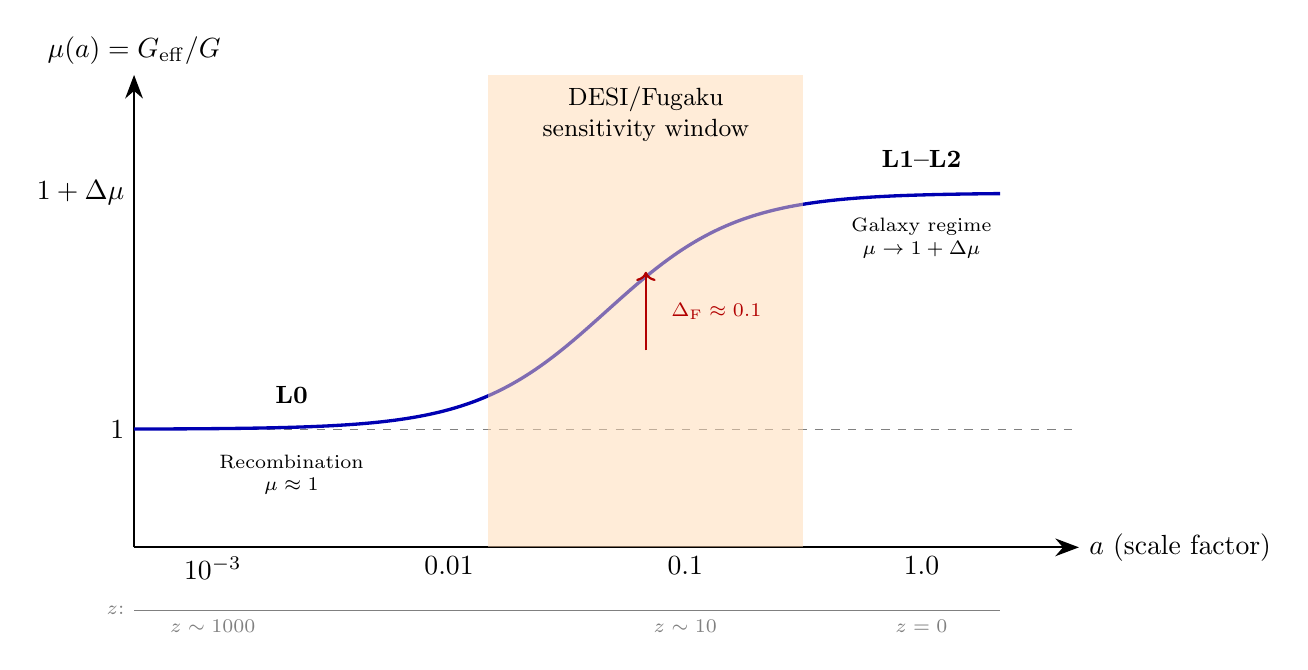
\begin{tikzpicture}[scale=1.0]
    % Axes
    \draw[-{Stealth[length=3mm]},thick] (0,0) -- (12,0) node[right] {$a$ (scale factor)};
    \draw[-{Stealth[length=3mm]},thick] (0,0) -- (0,6) node[above] {$\mu(a) = \Geff/G$};
    
    % Axis labels
    \node[below] at (1,0) {$10^{-3}$};
    \node[below] at (4,0) {$0.01$};
    \node[below] at (7,0) {$0.1$};
    \node[below] at (10,0) {$1.0$};
    
    % Horizontal reference line at mu=1
    \draw[dashed,gray] (0,1.5) -- (12,1.5);
    \node[left] at (0,1.5) {$1$};
    \node[left] at (0,4.5) {$1+\Deltamu$};
    
    % Transition curve
    \draw[very thick,blue!70!black,smooth] 
        plot[domain=0:11,samples=100] 
        (\x,{1.5 + 3/(1 + exp(-1.2*(\x - 6)))});
    
    % L0 regime label
    \node[above,font=\small\bfseries] at (2,1.7) {L0};
    \node[below,font=\scriptsize,align=center] at (2,1.3) {Recombination\\$\mu \approx 1$};
    
    % Transition band (shaded)
    \fill[orange!30,opacity=0.5] (4.5,0) rectangle (8.5,6);
    \node[font=\small,align=center] at (6.5,5.5) {DESI/Fugaku\\sensitivity window};
    
    % L1-L2 regime label
    \node[above,font=\small\bfseries] at (10,4.7) {L1--L2};
    \node[below,font=\scriptsize,align=center] at (10,4.3) {Galaxy regime\\$\mu \to 1+\Deltamu$};
    
    % Annotations
    \draw[->,thick,red!70!black] (6.5,2.5) -- (6.5,3.5);
    \node[right,font=\scriptsize,red!70!black] at (6.7,3) {$\DeltaF \approx 0.1$};
    
    % Redshift axis (secondary)
    \draw[gray] (0,-0.8) -- (11,-0.8);
    \node[below,font=\scriptsize,gray] at (1,-0.8) {$z \sim 1000$};
    \node[below,font=\scriptsize,gray] at (7,-0.8) {$z \sim 10$};
    \node[below,font=\scriptsize,gray] at (10,-0.8) {$z = 0$};
    \node[left,font=\scriptsize,gray] at (0,-0.8) {$z$:};
    
\end{tikzpicture}
\caption{\textbf{The regime-dependent effective gravitational coupling} $\mu(a) \equiv \Geff/G$ as a function of scale factor $a$ (or redshift $z$). At early times (L0, recombination epoch), $\mu \approx 1$ forms a flat plateau consistent with Planck CMB constraints. At late times and small scales (L1--L2, galaxy regime), $\mu$ asymptotically approaches a constant value $\mu > 1$ compatible with galaxy rotation curve phenomenology without additional matter components. The intermediate region defines a transition band in which $\mu(a)$ increases smoothly, parameterized by a bounded transition kernel. The shaded band denotes the DESI/Fugaku sensitivity window, within which Fugaku-class N-body simulations, when interpreted under DESI-calibrated parameter sets, exhibit an $\approx$10\% matter density offset relative to Planck $\Lambda$CDM. In the present framework, this offset is reinterpreted as an estimator of the integrated transition strength,
\begin{equation*}
\DeltaF = \int W(a)\,[\mu(a)-1]\,d\ln a,
\end{equation*}
where $W(a)$ represents the observational growth and BAO sensitivity kernel of DESI. The Fugaku offset therefore constrains the transition metric $\DeltaF$ rather than a fundamental density parameter. This single transition function simultaneously satisfies CMB consistency, large-scale structure growth constraints, and galaxy-scale phenomenology, enabling direct implementation in existing Boltzmann and structure solvers.}
\label{fig:transition}
\end{figure}

\newpage

% ===== Methods =====
\section{Methods: Transition Kernel and Estimator Definition}

\subsection{Effective Gravitational Coupling}

We parameterize deviations from standard growth behavior using the dimensionless effective coupling
\begin{equation}
\mu(a) \equiv \frac{\Geff(a)}{G},
\label{eq:mu_def}
\end{equation}
a standard phenomenological quantity used to encode scale- or time-dependent growth enhancement without introducing new background degrees of freedom.

\subsection{Transition Kernel}

The regime transition is modeled as a smooth, bounded function in log-scale factor:
\begin{equation}
\mu(a) = 1 + \Deltamu \; \mathcal{R}\!\left(\frac{\ln a - \ln a_t}{\sigma}\right),
\label{eq:transition_kernel}
\end{equation}
where
\begin{itemize}[leftmargin=2em,itemsep=0.3em]
    \item $a_t$ denotes the central transition epoch,
    \item $\sigma$ sets the transition width, and
    \item $\mathcal{R}(x)$ is a monotonic regulator (e.g., sigmoid or tanh) satisfying $\mathcal{R}(-\infty) = 0$, $\mathcal{R}(+\infty) = 1$.
\end{itemize}
The amplitude $\Deltamu$ is fixed by the Fugaku-derived estimator $\DeltaF$ and is not treated as a free function once calibrated.

\subsection{Transition Metric (Estimator)}

The integrated transition strength is defined as
\begin{equation}
\DeltaF \equiv \int_{a_{\min}}^{a_{\max}} W(a)\,[\mu(a)-1]\,d\ln a,
\label{eq:estimator}
\end{equation}
where $W(a)$ is a positive, normalized sensitivity kernel representing the redshift dependence of DESI growth and BAO constraints. The precise functional form of $W(a)$ is not required for the definition of the estimator, provided it is localized within the observational window of the simulations.

In Fugaku-class N-body simulations interpreted under DESI-calibrated parameter sets, the observed $\approx$10\% matter density offset relative to Planck $\Lambda$CDM corresponds to $\DeltaF \approx 0.1$, identifying the simulations as measurements of the integrated transition strength rather than of a fundamental density parameter.

\subsection{Consistency Conditions}

A valid transition function $\mu(a)$ must satisfy:

\begin{enumerate}[leftmargin=2em,itemsep=0.5em]
    \item \textbf{CMB Consistency:} $\mu(a) \to 1$ for $a \ll a_t$, preserving recombination-era constraints.
    
    \item \textbf{Large-Scale Structure Consistency:} $\DeltaF$ must match the Fugaku/DESI-inferred offset.
    
    \item \textbf{Galaxy-Scale Consistency:} $\mu(a) \to 1 + \Deltamu$ at late times, yielding the effective enhancement required by galaxy rotation curve phenomenology without introducing additional matter components.
\end{enumerate}

% ===== Acknowledgments =====
\section*{Acknowledgments}

This work was developed within the Energy-Flow Cosmology (EFC) framework. The author thanks the DESI and Fugaku simulation teams for making their results publicly available.

% ===== References =====
\section*{References}

\begin{enumerate}[leftmargin=2em,label={[\arabic*]},itemsep=0.3em]
    \item DESI Collaboration, \textit{DESI 2024 VI: Cosmological Constraints from the Measurements of Baryon Acoustic Oscillations}, arXiv:2404.03002 (2024).
    
    \item Planck Collaboration, \textit{Planck 2018 results. VI. Cosmological parameters}, A\&A 641, A6 (2020).
    
    \item Ishiyama, T., et al., \textit{The Uchuu simulations: Data Release 1 and dark matter halo concentrations}, MNRAS 506, 4210 (2021). [Fugaku N-body baseline]
    
    \item Magnusson, M., \textit{Foundations of Energy-Flow Cosmology (EFC): Regime Architecture and Methodological Principles of Entropy-Bounded Empiricism}, Figshare (2026). DOI: \href{https://doi.org/10.6084/m9.figshare.31135597}{10.6084/m9.figshare.31135597}.
    
    \item Magnusson, M., \textit{EFC Phenomenology vs DESI DR2 BAO: A Comparative Fit Analysis}, Figshare (2026). DOI: \href{https://doi.org/10.6084/m9.figshare.31127380}{10.6084/m9.figshare.31127380}.
    
    \item Magnusson, M., \textit{EFC Regime Transition Framework: A CMB-Consistent Approach to Late-Time Cosmology}, Figshare (2026). DOI: \href{https://doi.org/10.6084/m9.figshare.31096951}{10.6084/m9.figshare.31096951}.
    
    \item Magnusson, M., \textit{L0--L3 Regime Architecture in Entropy-Bounded Empiricism}, Figshare (2026). DOI: \href{https://doi.org/10.6084/m9.figshare.31112536}{10.6084/m9.figshare.31112536}.
    
    \item Magnusson, M., \textit{Systematic CMB Constraints on Early-Universe Modifications: Parameter Degeneracies and Null Results}, Figshare (2026). DOI: \href{https://doi.org/10.6084/m9.figshare.31095466}{10.6084/m9.figshare.31095466}.
    
    \item Magnusson, M., \textit{Comprehensive analysis of 175 SPARC galaxies demonstrating regime-dependent validity in rotation curve modeling}, Figshare (2026). DOI: \href{https://doi.org/10.6084/m9.figshare.31045126}{10.6084/m9.figshare.31045126}.
\end{enumerate}

\end{document}
